% =====================================================================
% ARQUITECTURA DEL SISTEMA. Explica con tus palabras cada componente y cómo se comunican:
%  - Dispositivos y Open Connect (el video sale de servidores dentro del proveedor de internet) \cite{Netflix_OpenConnect}
%  - AWS: ELB -> API Gateway (Zuul) -> Application API (Signup, Discovery, Play)
%  - Hystrix (cortacircuitos), microservicios con varias copias, Eureka (registro y latidos) \cite{SpringCloudNetflix}
%  - Datos: Cassandra / EVCache
%  - De dónde viene: Netflix migró de un monolito a microservicios (usa tus fichas \cite{Abgaz_2023} y \cite{Oumoussa_2024})
%  - Evolución del diagrama: primero el esquema a mano (Anexo A) y luego este en draw.io. ¿Qué agregaste y por qué?
% =====================================================================
\section{Arquitectura del sistema}

\textit{[Escribe aquí la descripción de la arquitectura.]}

\begin{figure}[H]
  \centering
  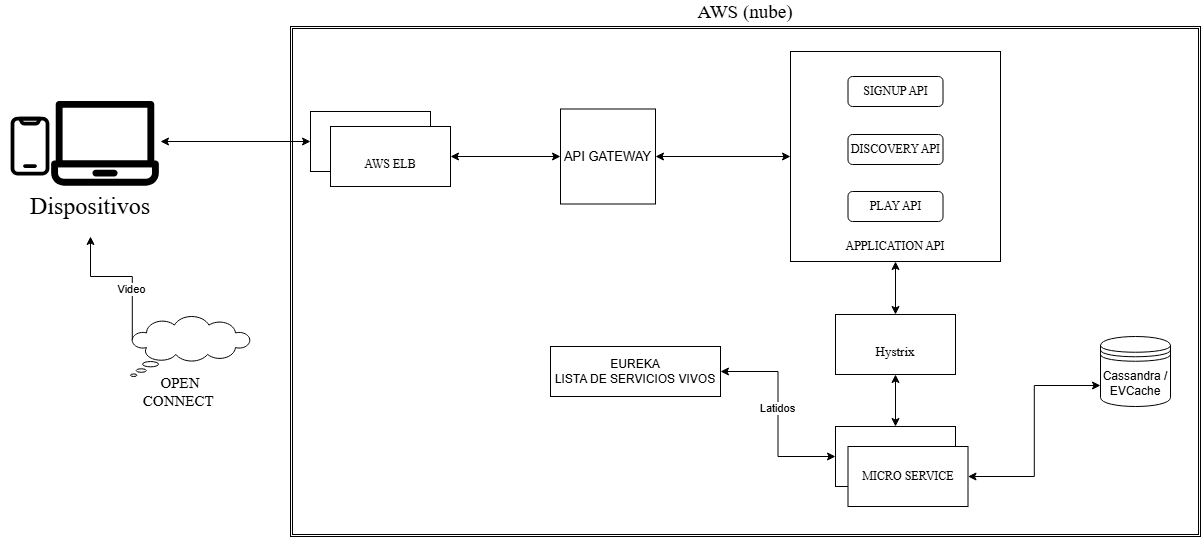
\includegraphics[width=\textwidth]{arquitectura.drawio.png}
  \caption{Arquitectura simplificada de Netflix, elaborada por el autor en draw.io a partir del esquema a mano del Anexo~A.}
  \label{fig:arquitectura}
\end{figure}

\textit{[Escribe aquí cómo evolucionó el diagrama desde el esquema a mano.]}
